\documentclass{article}
\usepackage[utf8]{inputenc}
\usepackage{url}
\def\UrlFont{\em}
\usepackage{indentfirst}

\title{Trabalho de Visão Relatório}
\author{Felipe Leivas Machado - 262528 \and Priscila Cavalli Rachevsky - 261573 }
\date{September 2019}

\usepackage{natbib}
\usepackage{graphicx}

\begin{document}

\maketitle

\section{Questão 1}
    Nesta questão precisavamos desenhar uma linha para representar um jogador que estaria num certo ponto (X,Y), onde X e Y representam o pixel dos pés do jogador. Para podermos fazer isso precisavamos calcular algumas coisas, como:
   \begin{itemize}
       \item Gerar os pontos de calibragem
       \item Gerar a matriz P de calibragem da camera
       \item Converter uma coordenada 2D para uma cordenada 3D
       \item Converter uma coordenada 3D  para uma cordenada 2D
       \item Desenhar uma reta entre dois pontos
   \end{itemize}

    \subsection{Geração dos pontos}
        Para gerar os pontos pegamos alguns pontos fáceis de calcular a sua posição no mundo real. Os pontos selecionados estão destacados em vermelho, já o centro da imagem é o ponto azul:

        \begin{figure}[h!]
        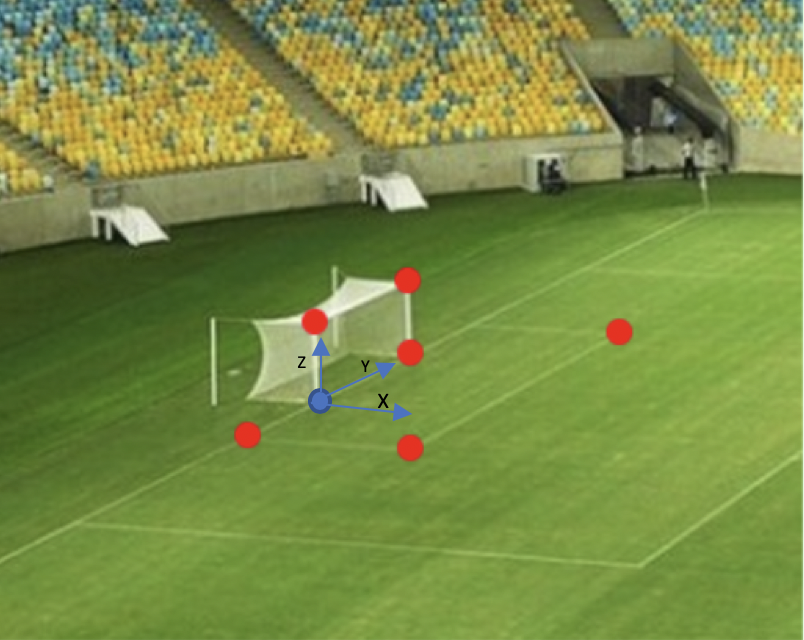
\includegraphics[scale=0.5]{maracana1Pontos.png}
        \end{figure}
    \subsection{Geração da Matriz de calibragem}
    Para geração da matriz de calibragem, primeiramente foi gerada a matriz A com base nos 6 pontos selecionados

\section{Questão 2}
    Desenhar uma linha no campo paralela à de impedimento, para isso foi necessário fazer os seguintes passos:
   \begin{itemize}
       \item Coleta dos pontos de calibragem
       \item Descobrir matriz da câmera
       \item Desenhar uma reta entre dois pontos
   \end{itemize}

    \subsection{Coleta dos pontos de calibragem}
    Da mesma forma que no exercício passado, a coleta dos pontos na imagem foi feita manualmente e depois calculados conforme a nova origem, já para achar os respectivos pontos no mundo real, se usou a definição do trabalho com o tamanho do campo. Mas ao contrário do exercício anterior, não foi preciso escolher pontos em que a coordenada Z fosse diferente de 0, porque nesse exercício se usou estratégia de calibragem \textit{plane to plane}. Além disso provou-se que apenas 4 pontos já era o suficiente.
    
    Na Figure ~\ref{fig:maracana2Pontos} pode-se ver os 4 pontos escolhidos em vermelho, em amarelo a origem e a orientação das coordenadas.
        \begin{figure}[h!]
        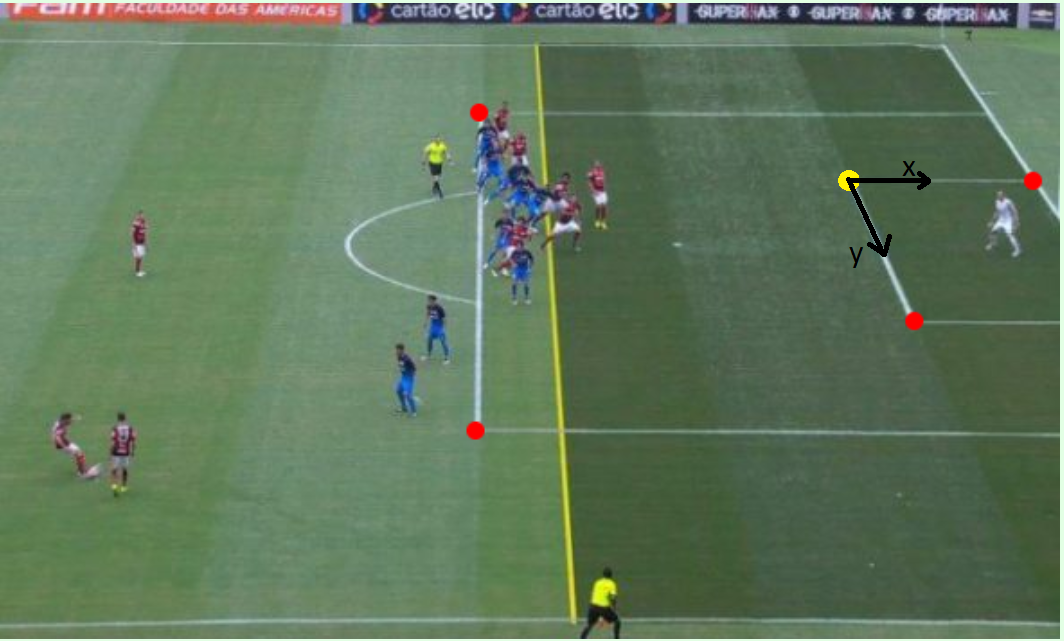
\includegraphics[scale=0.6]{maracana2Pontos.PNG}
        \caption{Em vermelho os 4 pontos escolhidos e em amarelo a origem}
        \label{fig:maracana2Pontos}
        \end{figure}
        
    \subsection{Descobrir matriz da câmera}
    Para descobrir a matriz da câmera deve-se descobrir a matriz P. Então, reutilizou as estratégia da questão anterior, modificando a equação como mostra a Figure ~\ref{fig:planeToPlane}.
    \begin{figure}[h!]
    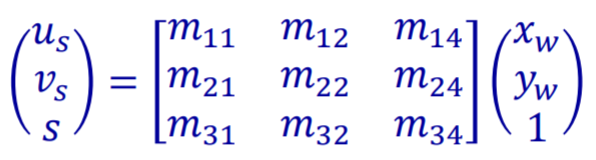
\includegraphics[scale=0.6]{planeToPlane.PNG}
    \caption{O modelo matemático para calibragem \textit{plane to plane}}
    \label{fig:planeToPlane}
    \end{figure}
        
        \subsection{Matriz A}
        A matriz A foi modificada para ter o tamanho 9x4, já que retirou-se as três colunas que eram associadas à coordenada Z e usou-se apenas 4 pontos, como mencionado anteriormente. (Figure ~\ref{fig:matrizA})
        
        \begin{figure}[h!]
        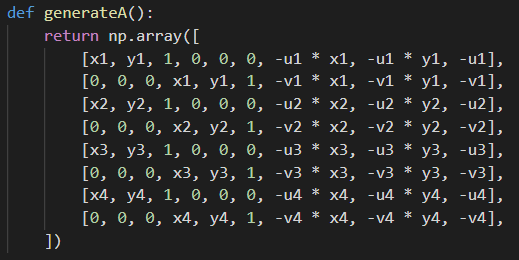
\includegraphics[scale=1]{matrizA.PNG}
        \caption{Matriz A para calibragem \textit{plane to plane}}
        \label{fig:matrizA}
        \end{figure}
        
        \subsection{Matriz P}
        Fez-se \textit{svd} na Matriz A, então pegou a última matriz de V e se fez o \textit{reshape} para ficar do tamnho 3x3. (Figure ~\ref{fig:matrizP})
        
        \begin{figure}[h!]
        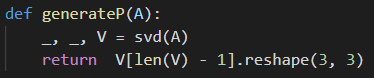
\includegraphics[scale=1]{matrizP.PNG}
        \caption{Matriz P a partir da matriz A}
        \label{fig:matrizP}
        \end{figure}
        
    \section{Desenhar uma reta entre uma lateral a outra}
    Tem diversas formas de desenhar linhas paralelas a do impedimento, nesse trabalho escolheu-se a solução em que desenhava uma reta de uma lateral a outra. 
    
    Assim, só precisou descobrir os pontos das laterais. Implementou-se dessa forma: dado um ponto clicado na imagem e calculado no sistema 2D, descobria-se seu respectivo ponto Pm no mundo real (Figure ~\ref{fig:calculateRealWorldPoint}), e então, descobria os dois pontos em cada lateral (Pl1 e Pl2) fazendo Pl1 = (Pm[x], lateralDeCimaY) e Pl2 = (Pm[x], lateralDeBaixoY). Porém, a imagem da definição do trabalho não deixava claro qual o tamanho exato do campo (de 45 a 90m), então, também coletados manualmente, dois pixels localizados cada um em uma lateral e transformados em pontos do mundo real, então descobriu que a quadra tem aproximadamente 67m. Dessa forma, sabendo a origem, foi possível calcular o valor de lateralDeCimaY e lateralDeBaixoY.
    
        \begin{figure}[h!]
        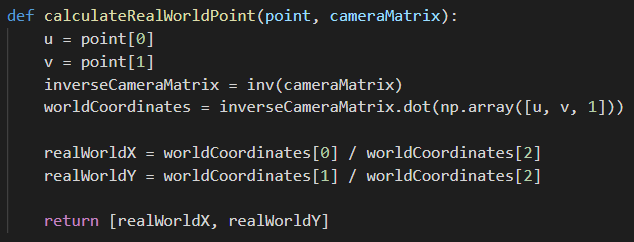
\includegraphics[scale=0.9]{calculateRealWorldPoint.PNG}
        \caption{Função que calcula o ponto no mundo real dado o ponto na imagem e a matriz da câmera}
        \label{fig:calculateRealWorldPoint}
        \end{figure}
        
    A Figure ~\ref{fig:result2} é o resultado do execício, pode se ver que não ficou perfeitamente paralelo a linha da pequena área, mas consideramos um resultado satisfatório.
        \begin{figure}[h!]
        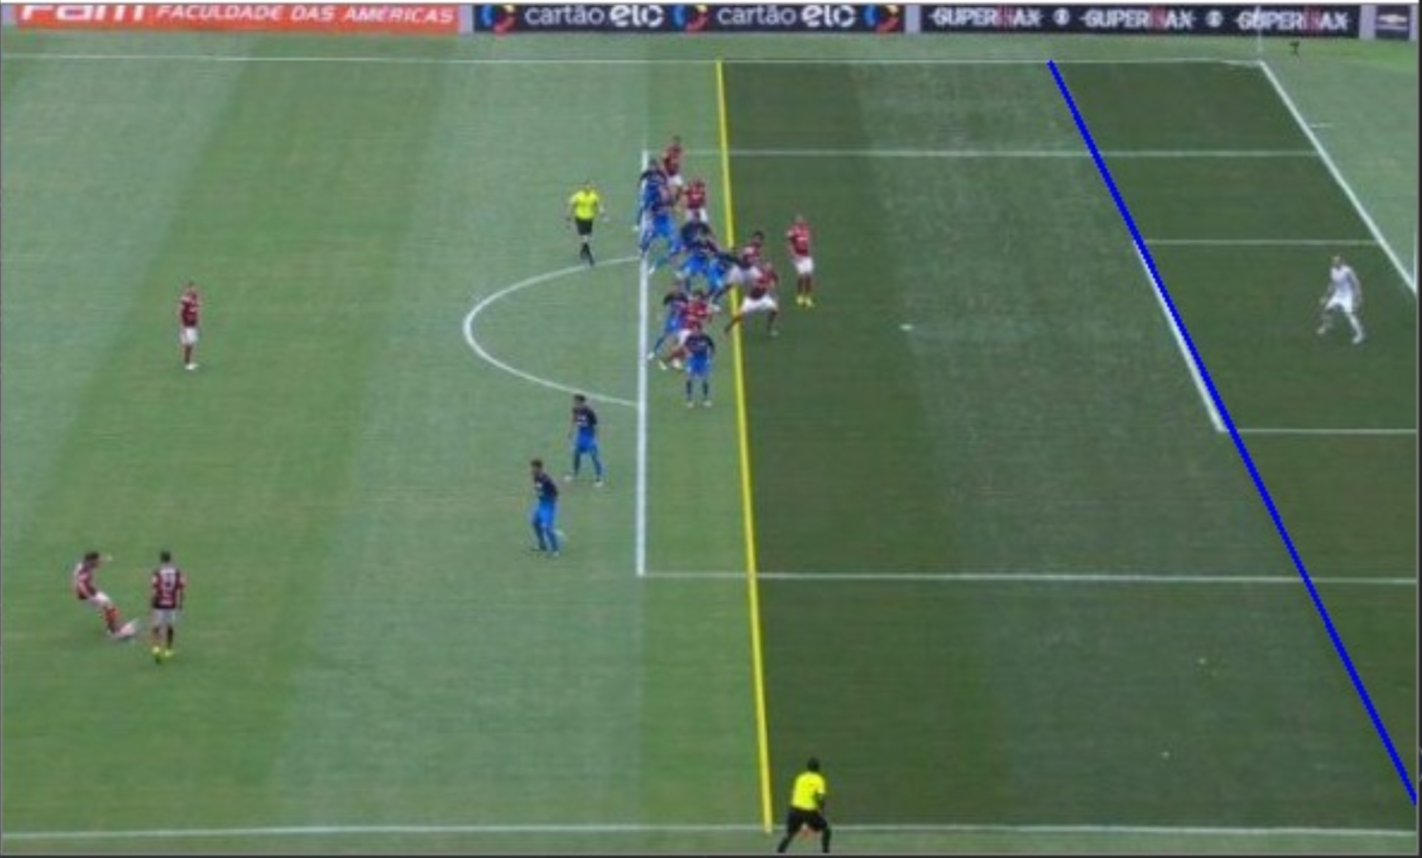
\includegraphics[scale=0.5]{result2.PNG}
        \caption{Função que calcula o ponto no mundo real dado o ponto na imagem e a matriz da câmera}
        \label{fig:result2}
        \end{figure}
    

\section{Conclusão}
``I always thought something was fundamentally wrong with the universe'' \citep{adams1995hitchhiker}

\bibliographystyle{plain}
\bibliography{references}
\end{document}
